\documentclass[]{elsarticle}
\usepackage[latin1]{inputenc}
\usepackage{graphicx}
\usepackage[left=1.00in, right=1.00in, top=1.10in, bottom=1.00in]{geometry}

\usepackage{dirtytalk}
\usepackage[normalem]{ulem}
\usepackage{tikz-cd}
\usepackage{units}
\usepackage{algorithm}
\usepackage{algpseudocode}
\usepackage{alltt}
\usepackage{mathrsfs}
\usepackage{amssymb}
\usepackage{amsmath}
\DeclareMathOperator\cis{cis}

% (font shortcuts)
\usepackage{amsfonts}
\newcommand{\mb}[1]{\mathbb{#1}}
\newcommand{\mc}[1]{\mathcal{#1}}
\newcommand{\ms}[1]{\mathscr{#1}}
\newcommand{\mf}[1]{\frak{#1}}

% (arrow shortcuts)
\newcommand{\ra}{\rightarrow}
\newcommand{\lra}{\longrightarrow}
\newcommand{\la}{\leftarrow}
\newcommand{\lla}{\longleftarrow}
\newcommand{\Ra}{\Rightarrow}
\newcommand{\Lra}{\Longrightarrow}
\newcommand{\La}{\Leftarrow}
\newcommand{\Lla}{\Longleftarrow}
\newcommand{\lr}{\leftrightarrow}
\newcommand{\llr}{\longleftrightarrow}
\newcommand{\Lr}{\Leftrightarrow}
\newcommand{\Llr}{\Longleftrightarrow}

% (match parenthesis)
\newcommand{\mlr}[1]{\left|#1\right|}
\newcommand{\plr}[1]{\left(#1\right)}
\newcommand{\blr}[1]{\left[#1\right]}

% (exponent shortcuts)
\newcommand{\inv}{^{-1}}
\newcommand{\nrt}[2]{\sqrt[\leftroot{-2}\uproot{2}#1]{#2}}

% (annotation shortcuts)
\newcommand{\conj}[1]{\overline{#1}}
\newcommand{\ol}[1]{\overline{#1}}
\newcommand{\ul}[1]{\underline{#1}}
\newcommand{\os}[2]{\overset{#1}{#2}}
\newcommand{\us}[2]{\underset{#1}{#2}}
\newcommand{\ob}[2]{\overbrace{#2}^{#1}}
\newcommand{\ub}[2]{\underbrace{#2}_{#1}}
\newcommand{\bs}{\backslash}
\newcommand{\ds}{\displaystyle}

% (set builder)
\newcommand{\set}[1]{\left\{ #1 \right\}}
\newcommand{\setc}[2]{\left\{ #1 : #2 \right\}}
\newcommand{\setm}[2]{\left\{ #1 \, \middle| \, #2 \right\}}

% (group generator)
\newcommand{\gen}[1]{\langle #1 \rangle}

% (functions)
\newcommand{\im}[1]{\text{im}(#1)}
\newcommand{\range}[1]{\text{range}(#1)}
\newcommand{\domain}[1]{\text{domain}(#1)}
\newcommand{\dist}[1]{(#1)}
\newcommand{\sgn}{\text{sgn}}

% (Linear Algebra)
\newcommand{\mat}[1]{\begin{bmatrix}#1\end{bmatrix}}
\newcommand{\pmat}[1]{\begin{pmatrix}#1\end{pmatrix}}
%\newcommand{\dim}[1]{\text{dim}(#1)}
\newcommand{\rnk}[1]{\text{rank}(#1)}
\newcommand{\nul}[1]{\text{nul}(#1)}
\newcommand{\spn}[1]{\text{span}\,#1}
\newcommand{\col}[1]{\text{col}(#1)}
%\newcommand{\ker}[1]{\text{ker}(#1)}
\newcommand{\row}[1]{\text{row}(#1)}
\newcommand{\area}[1]{\text{area}(#1)}
\newcommand{\nullity}[1]{\text{nullity}(#1)}
\newcommand{\proj}[2]{\text{proj}_{#1}\left(#2\right)}
\newcommand{\diam}[1]{\text{diam}\,#1}

% (Vectors common)
\newcommand{\myvec}[1]{\vec{#1}}
\newcommand{\va}{\myvec{a}}
\newcommand{\vb}{\myvec{b}}
\newcommand{\vc}{\myvec{c}}
\newcommand{\vd}{\myvec{d}}
\newcommand{\ve}{\myvec{e}}
\newcommand{\vf}{\myvec{f}}
\newcommand{\vg}{\myvec{g}}
\newcommand{\vh}{\myvec{h}}
\newcommand{\vi}{\myvec{i}}
\newcommand{\vj}{\myvec{j}}
\newcommand{\vk}{\myvec{k}}
\newcommand{\vl}{\myvec{l}}
\newcommand{\vm}{\myvec{m}}
\newcommand{\vn}{\myvec{n}}
\newcommand{\vo}{\myvec{o}}
\newcommand{\vp}{\myvec{p}}
\newcommand{\vq}{\myvec{q}}
\newcommand{\vr}{\myvec{r}}
\newcommand{\vs}{\myvec{s}}
\newcommand{\vt}{\myvec{t}}
\newcommand{\vu}{\myvec{u}}
\newcommand{\vv}{\myvec{v}}
\newcommand{\vw}{\myvec{w}}
\newcommand{\vx}{\myvec{x}}
\newcommand{\vy}{\myvec{y}}
\newcommand{\vz}{\myvec{z}}
\newcommand{\vzero}{\myvec{0}}

% Theorems and Propositions
\usepackage{amsthm}
\newtheorem{theorem}{Theorem}
\newtheorem{proposition}{Proposition}

\theoremstyle{definition}
\newtheorem{definition}{Definition}

\theoremstyle{remark}
\newtheorem*{remark}{Remark}
\newtheorem{example}{Example}
\newtheorem*{recall}{Recall}
\newtheorem*{note}{Note}
\newtheorem*{observe}{Observe}
\newtheorem*{question}{\underline{Question}}
\newtheorem*{fact}{Fact}
\newtheorem{corollary}{Corollary}
\newtheorem*{lemma}{Lemma}
\newtheorem{xca}{Exercise}

%\usepackage[active,tightpage]{preview}
\setlength\PreviewBorder{7.77pt}
\usepackage{varwidth}
\AtBeginDocument{\begin{preview}\begin{varwidth}{\linewidth}}
\AtEndDocument{\end{varwidth}\end{preview}}


\usepackage{subcaption}
\usepackage{stmaryrd}

%\usepackage{fontspec}
%\setmainfont{Latin Modern Math}

\journal{Advances in Engineering Software}
\bibliographystyle{elsarticle-num}

%% Group authors per affiliation:
%\author{Elsevier\fnref{myfootnote}}
%\fntext[myfootnote]{Since 1880.}

\begin{document}
\begin{frontmatter}
\author{Michael Reed}%\fntext{myfootnote}}
\address{Crucial Flow Research}
%\fntext[myfootnote]{Computational Meta-Linguist}
\title{Optimal polynomial form characteristic methods}
%\date{October 19, 2018}

%\maketitle
%floating-point product, universal algebra, rounding error analysis, polynomial evaluation, Horner scheme, Wilkinson type error estimates, IEEE 754 standard
\begin{abstract}
There are several possible forms for a polynomial expression's terms, such as factored form, expanded form, Horner form, and many others.
The set of such possible forms is an equivalence class of a universal algebra. However, when the operations are replaced with floating point pseudo-operations, the equivalence relation on the terms no longer holds and a rounding error is introduced.
For each polynomial the computational effort and numerical error can be reduced with a form that is equivalent on the dense polynomial algebra by using a comparison of characteristic values. A local and a global theory of characteristic values is investigated to select the appropriate form on a given floating point interval.
%Additionally, a Julia language package is provided to allow researchers to test and analyze their own polynomial examples.
%Let $f$ be an expression term of a function $y(x)=f$. %and let $c(f)$ be the number of $f$'s operation and function calls. v
%There are several possible forms for a polynomial expression terms, such as factored form $\mc F(f)$, expanded form $\mc E(f)$, and Horner form $\mc H(f)$. The set of such possible forms is denoted $\ms E(f)=\set{f,\mc F(f),\mc E(f),\mc H(f),\dots}$.
%Each form of $f$ will typically have a different value for $c(\mc F(f))$ and $c(\mc H(f))$,.
%For each polynomial the computational effort and numerical error can be minimized with a form of $f$ by comparison of characteristic values.
%can be computed with a lower number of floating point operations in $\mc H$ form or in $\mc F$ form, depending on the roots of that polynomial.
\end{abstract}

%\begin{keyword}
%\texttt{elsarticle.cls}\sep \LaTeX\sep Elsevier \sep template
%\MSC[2010] 00-01\sep  99-00
%\end{keyword}

\end{frontmatter}

%In the mathematical literature there is not yet much 
The goal of this paper is to propose and investigate a variety of characteristic criteria concerning the selection of optimal polynomial forms.
In this paper, optimization criteria based on local and global characteristics will be investigated.
In the past, it has been discussed that the Horner form of a polynomial is the optimal solution if only the number of operations is minimized \cite{borodin}.
Operation count is the only global characteristic which is currently used to identify the Horner form as optimal for general cases.
Additional global characteristics will be introduced in this paper.

The local characteristics are based off of the locally compounded rounding errors from polynomial evaluation on a floating point pseudo-algebra, which has been pioneered by Wilkinson \cite{wilkinson}.
Several bounds for the error in the evaluation of the Horner form of a polynomial have been proved \cite{muller}\cite{rump-bunger-jeannerod} and it has been shown that the Chebyshev form has worse error propagation characteristics than the Horner form \cite{newbery}\cite{oliver}.
There have also been some investigation of unified rounding error bounds for polynomial evaluation of forms in an arbitrary polynomial basis \cite{barrio}.
What has not been investigated yet is the error bound for any term of a universal algebra for polynomials, including arbitrary trees of operations that need not be in Horner form or basis form.
This paper seeks to provide the theoretical terminology to express this error bound and to use it for a local and global characteristic analysis in polynomial form optimization.

\section{Universal algebra for polynomials}

A (universal) algebra \cite{sapir} for polynomials $\mb P$ is a set $\mb K$ with the closed operations $\set{+,-,\times,/,\widehat{\ \ }}$, with operations $+,-,\times$ being mappings of the kind $\mb K^2\ra\mb K$ and $/,\widehat{\ \ }$ being maps of the kind $\mb K\times\mb Z\ra\mb K$. The algebra is denoted $\mb P(\mb K)=(\mb K,\set{+,-,\times,/,\widehat{\ \ }})$. Examples are $\mb P(\mb F_p),\mb P(\mb Q),\mb P(\mb R)$, and $\mb P(\mb C)$.
\begin{definition}
	[Term] The composition of several basic operations of an algebra $(\mb K,O)$ is called a term.
	An abstract syntax tree of a polynomial term $f$ is a directed rooted graph representing the functional structure of the expression.
	Let $c(f)$ be the number of operations in $f$'s abstract syntax tree, % and function calls.
	let $G(f)=\set{g_1,\dots,g_*}$ be the set of constant scalars used in $f$.
	Each vertex $v_j(x,g_*,\dots,v_*)\in V(f)$ along the graph represents a function value recursively obtained from input leaves (scalar constants $g_j\in G(f)$ or the variable $x$) or the result from nested vertices $v_*\in V(f)$, thus $c(f) = |V(f)|$. A term $f$ is also a function on the set $\mb K$ and
	\begin{align*}
		f &= v_*(x,g_*,\dots,v_*(x,g_*,\dots,v_*(x,g_*,\dots),\dots,v_*(x,g_*,\dots)),\dots,v_*(x,g_*,\dots)), \qquad v_j &\mapsfrom \begin{cases} x\in\mb K \\ g_*\in G(f)\\ v_*\in V(f) \end{cases}.
	\end{align*}
\end{definition}
\begin{definition}
	Let $P(f)=\set{p_1,\dots,p_m}$ be the set of all power exponents $p_i$ in the polynomial expression $f$ such that $p_i\neq 0,1$, and let $S(f)=\set{s_1,\dots,s_n}$ be the set of all other coefficient scalars in~$f$.
	%The sets $P(f),S(f)$ and the vertex degree of the tree $c(f)$ help characterize the bounds on the numerical error estimate. %, as explained later.
	%$$ d(x,i) = \begin{cases} |x|\cdot d(x,i+1) + |a_i| & i < n \\ |a_n| & i = n \end{cases} $$
	%Horner's rule:
	%$r_n(x) = p(n-1,a_n,x)$ with $p(n,\alpha,x) = a_n + \alpha x$ and $p(0,\alpha,x)=a_0$
\end{definition}
The Horner form of a polynomial $\mc H(f)\equiv h_f(x,0)$ is defined as a recursive chain of vertices $$ h_f(x,j) = \begin{cases} +(\times( h_f(x,j+1),x),s_j), & 0 \leq j < n \\ s_n, & j = n \end{cases},$$
thus forming a nested alternating sequence of binary floating point operations. 
The expanded form and Horner form of a polynomial both use the same \cite{epperson} coefficients $S(\mc E(f))\equiv S(\mc H(f))$, and are related by 
\begin{align*}
	\mc H(f) \equiv +(\times(+(...+(\times(+(\times(s_n,x),s_{n-1}),x),\dots),s_1),x),s_0) 
	&=\Sigma\plr{\times(\widehat{\ \ }(x,j),s_j),j,1,n} \\
	= +(\times(\widehat{\ \ }(x,0),s_0), \dots, \times(\widehat{\ \ }(x,j),s_j), \dots ,\times(\widehat{\ \ }(x,n),s_n)
	&= \sum_{j=0}^ns_jx^j \equiv \mc E(f)
\end{align*}
Note that $P(\mc H(f)) = \emptyset$ and $P(\mc E(f))\subset\set{2,\dots,|S(\mc E(f))|+1}$ for any polynomial $f$.

Another possible form of $f$ is guaranteed by the fundamental theorem of algebra, which tells us that any polynomial with complex coefficients has $n$ roots $r_j\in\mb C$, where $$ \mc F(f) \equiv \prod_{j=1}^n (x-r_j) = \Pi(-(x,r_j),j,1,n) = \times(-(x,r_1),\dots,-(x,r_j),\dots,-(x,r_n)) $$

% (((x - 2) ^ 2 * x ^ 2 - 1) ^ 2 - 1) ^ 2
\begin{example}
	Consider an expression $f$ such that $\mc E(f) = 4x^4-44x^3+61x^2+270x-525$. Then the corresponding sets are $S(\mc E(f)) = \set{4,-44,61,270,-525}$ and $P(\mc E(f)) = \set{4,3,2}$, while the Horner form has $P(\mc H(f)) = \emptyset$. 
	For the factorized form, $P(f) = \set{2_1,2_2}$ and $S(f) = \set{-6,-21,2,-5}$. Figure \ref{graph-tree} shows the different forms.
	Note that in this case, a fully factored form $\mc F(f)$ was not obtained, as it is inaccessible to the algorithm.
\end{example}

\begin{figure}[hb]
	\centering
	\includegraphics{figs/ast}
	%\hfill
	\caption{Abstract syntax trees of $\mc H(f),\mc E(f),\mc F(f)$ with vertices $v_j$ and leaves $x$ and $g_*$.}
	\label{graph-tree}
\end{figure}

Let $a(x),b(x)$ be terms of a polynomial algebra $\mb P(\mb K)$. Define a relation $\sim$ such that $a\sim b$ if and only if $a(x)=b(x)$ for all $x\in\mb K$. It is trivial to show that $\sim$ is an equivalence relation on $\mb P(\mb K)$, so there exists a partition of $\mb P(\mb K)$ into equivalence classes
$\ms E(f) := \set{a\in\mb P(\mb K):a\sim f}\in\mb P(\mb K)/\sim$.

Thus it is clear that $|\ms E(f)|\geq3$ for any non-trivial polynomial for which these base forms do not coincide. 
In fact, $|\ms E(f)|=\infty$ since there are infinite possibilities of rearranging the same polynomial's terms using cancellations. 
We will restrict ourselves to the forms accessible via algorithmic rewriting and remark that there are practically inaccessible forms. 
For example, it is not always possible to compute the factorized form of a polynomial in terms of a closed form expression, since irrational roots are possible.

\section{The floating point pseudo-algebra}

Recall that a floating point number is a value represented by a finte sequence of bits \cite{higham}.
Let $n$ be the number of bits assigned to the fractional mantissa $m$ and let $r$ be the number of bits assigned to the exponent $t$. 
Using a signed $1+n+r$ bit representation, floating point numbers have the form
$ x := \sgn(x)\cdot m \cdot 2^{t-s} $.
where $\sgn(x)$ is the sign of the number, $m$ is the mantissa $$m = \sum_{k\in B}2^{-k}$$ with $B\subseteq\set{1,\dots,n}$, and $t$ is an integer such that $0\leq t\leq 2^r-1$ with shift $s := 2^{r-1}-1$.
The set of bits (numbered from 1 to $n$) that are true in the mantissa is the set $B$.
\begin{definition}
	[Floating point set]
	The set of all floating point numbers that can be represented with an $n$-bit mantissa with and an $r$-bit exponential shift of $s=2^{r-1}-1$ is
	$$ \mb M(n,s) := \bigg\{x\in\mb Q\,\bigg|\,x = \pm\sum_{k\in B} 2^{t-s-k},B\subseteq\set{1,\dots,n},t\in\set{0,\dots,2s+1}\bigg\}\subset\mb R. $$
\end{definition}
Consider the 1 bit for $\sgn(x)$, $n$ bits for the mantissa, and $r$ bits for the exponent. Then it follows that $0\leq t\leq 2s+1 = 2^r-1$ implies $r = 1+\log_2(s+1)$ is the number of bits for the exponent.
Hence, the number of bits per floating point number is $2+n+\log_2(s+1)$.
The IEEE-754 standard for single precision 32-bit floating point is $\mb M(23,127)$ and it is $\mb M(52,1023)$ for 64-bit double precision.
For each bit there are two possibilities, therefore the size of a floating point set is $ |\mb M(n,s)| =2^{1+n+r} = 2^{2+n+\log_2(s+1)} = 4(s+1) 2^n$, which is finite.
%\begin{proposition}
%	The size of a floating point set is $|\mb M(n,s)| = 4(s+1)2^n$, which is finite.
%\end{proposition}
The main numerical difficulty we will encounter can be attributed to the fact that $|\mb M(n,s)|<|\mb Q|<|\mb R|$.

%Suppose that $a\sim b$ implies $a\sim|_{M(n,s)}\,b$.
It turns out that $\mb P(\mb M(n,s))$ is not a universal algebra, but rather must be considered a pseudo-algebra since the operations must be replaced with rounded pseudo-operations to be closed.
Let $x\in \mb M(n,s)\subset\mb Q$ and let $a\equiv (1+x)\cdot x$ and $b\equiv x+x^2$.
The following steps apply to positive values of $x$, but similar steps can be followed for a negative value.
Specifically, let $x = \sum_{k\in B} 2^{t-s-k}$ for some $B\subset\set{1,\dots,n}$ such that $t-s\notin B$ with $0\leq t\leq s$.
Then $1+x = \sum_{k\in B\cup\set{t-s}}2^{t-s-k}$ and $(1+x)\cdot x = \sum_{k\in\tilde B} 2^{t-s-k}$ for some $\tilde B$. If $\min B=1$, then $2t-2s-2\in\tilde B$. Then, $t-s-n>0$ implies that $2t-2s-2>2(n-1)$.
However, $\max B\leq n\leq2(n-1)$ implies that $2t-2s-2>\max B$.
Thus, rounding must be introduced by taking $\sum_{k\in\tilde B\cap\set{1,\dots,n}}2^{t-s-k}$ to approximate the nearest value of $(1+x)\cdot x$ in $\mb M(n,s)$.
Likewise, for $x+x^2$ it is possible for rounding to be introduced at each of the two operations (depending on $B$). Generally, the number and error of these roundings for the terms $a$ and $b$ need not be the same.
Therefore, the resulting values of evaluating $a(x)$ and $b(x)$ need not be equal for all $x\in\mb M(n,s)$.
%This means that $a\sim b$ does not imply $a\sim|_{\mb M(n,s)}\,b$.
%\begin{proposition}
%	Let $\sim|_{M(n,s)}$ be a restriction of the equivalence relation $\sim$ on the dense polynomial algebra $(\mb K,\set{+,-,\times,/,\widehat{\ \ }}$ with terms $a,b$ and $\mb K\in\set{\mb Q,\mb R}$. Then $a\sim b$ does not imply that $a\sim|_{M(n,s)}\,b$.
%\end{proposition}
	
Consequently, the equivalence relation $\sim$ does not hold for terms in $\mb P(\mb M(n,s))$ which would otherwise be in the same equivalence class for $\mb P(\mb K)$ with a dense set $\mb K$.
%\section{Local error theory}
%Therefore, it is clear that restricting ourselves from a dense set to $\mb M(n,s)$ does not generally preserve the equivalence relation $\sim$. 
This necessitates the introduction of the floating point error introduced by the rounding at each operation of the term of a polynomial algebra.
The machine epsilon upper bound of the relative error due to floating point rounding is $\epsilon:=2^{-n}$.
Let $\delta_j(x)$ be the the floating point round-off error at each operation $v_j$ such that $0\leq\delta_j(x)\leq\epsilon$ for all $x,j$.
The propagation of this error can be understood recursively by the term rewrite map $alg:\mb P(\mb K)\ra\mb P(\mb M(n,s))$ defined by
\begin{align*}
	alg(v_j) &:=
	(1+\delta_j(x))\cdot v_j(x,g_*,alg(v_1),\dots,alg(v_{c(f)})).
\end{align*}

%\section{Local theory of roundoff error}
Define $abs(f)$ to be the expression transformation that replaces all elements of $s_i\in S(f)$ with $|s_i|$, i.e. replace any non-exponent scalar with its modulus. Then $abs:V(f)\ra \mb P(\mb K)$ is the term rewrite function
\begin{align*}
	abs(v_j) &:= \begin{cases}
		+_j(|x|,|g_*|,abs(v_1),\dots,abs(v_{c(f)})) & \text{if }v_j =\, - \\
		\widehat{\,\,}\,_j(|x|,g_*,abs(v_1),\dots,abs(v_{c(f)})) & \text{if } v_j =\, \widehat{\ \ } \\
		v_j(|x|,|g_*|,abs(v_1),\dots,abs(v_{c(f)})) & \text{if } v_j \in V(f)\bs\set{-,\widehat{\ \ }} %\\
		%|g_*| & v_j \in G(f)
	\end{cases}.
\end{align*}
For example, $abs(4x^4-44x^3+61x^2+270x-525) = 4x^4+44x^3+61x^2+270x+525$.
Note that $\blr{abs(f)}(x)$ is the evaluation of this transformed expression at $x$.
For an expression based on a polynomial basis, it has been shown that the round-off error bound can be distributed over the operations and ultimately rearranged into expanded form \cite{demmel}. By rearrangement, a bound on the round-off error can be estimated at each $x$.

\begin{theorem}
	%It can be shown that 
	The maximum floating point error for evaluating $f=f(x)$ is bounded by
	\begin{align*}
		\delta(f,x,\epsilon) &= \epsilon\cdot c(f)\cdot \blr{\text{abs}(f)}(x), & \lim_{\epsilon\ra0}\delta(f,x,\epsilon) = 0,
	\end{align*}
	with property $\delta(f,x,\epsilon)>0$ for all $x\in(0,\infty)$ and $\epsilon>0$ for any non-trivial $f$. %(specifically for Horner form, but this generalizes)
\end{theorem}
\begin{proof}
	Take the expanded form of $alg(f)$ and note that there are at most $c(f)$ of $1+\delta_k(x)$, hence
	\begin{align*}
		\mc E(alg(f)) &\equiv \sum_{j=0}^n s_jx^j\prod_k(1+\delta_k(x)) \leq \sum_{j=0}^n s_j x^j (1+\epsilon)^{c(f)} \leq \sum_{j=0}^n s_jx^j(1+c(f)\cdot\epsilon), \\
		\mlr{f-\mc E(alg(f))} &\leq \mlr{\sum_{j=0}^n s_j x^j(1+c(f)\cdot\epsilon)-\sum_{j=0}^ns_jx^j} \leq \mlr{\sum_{j=0}^n s_j x^j c(f)\cdot \epsilon} \leq \epsilon\cdot c(f)\sum_{j=0}^n|s_j|\,|x|^j.
	\end{align*}
	Observe that this is equivalent to $\epsilon\cdot c(f)\cdot abs(\mc E(f)) \leq \epsilon\cdot c(f)\cdot abs(f) = \delta(f,x,\epsilon)$.
\end{proof}

%Consider $abs_\epsilon(f)$ such that $\delta_j(x)\equiv\epsilon$ for all $j,x$.
%Examples indicate that $\mc E(alg_\epsilon(g))\equiv\delta(f,x,\epsilon)$ exactly for all $g\in\ms E(f)$, which would imply that $\delta(f,x,\epsilon)$ is an ideal bound.
%However, due to the wide range of values that $x$ can take on with a floating point number system it is desirable to measure the data on logarithmic scales.
For each polynomial form, the calculation of the bound will be different due to variations in $c(f)$ and error propagation. 
The scaled error bound is $\delta(f,x,\epsilon)/|x|$
%We set $\epsilon>0$ as the machine epsilon value of the floating point computer 
and we denote $\Omega(f,\epsilon)$ as the maximum floating point value of $x$ before the evaluation for $f$ reaches the floating point ceiling.

\begin{figure*}[ht]
	\centering
	\caption{Graph of the scaled bound for the polynomial $f$}
	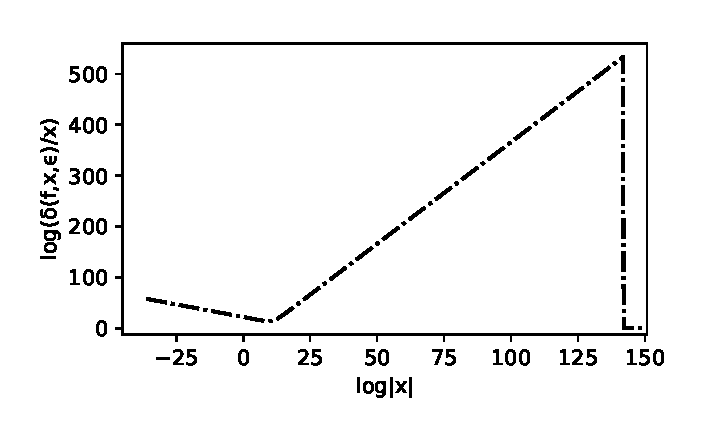
\includegraphics[width=0.54\linewidth]{figs/graph}
\end{figure*}

\section{Global characteristic methods}

In order to obtain a normalized comparison of each bound the average of the Stieltjes integeral can be obtained.
Then to measure the accumulation discrepancy $\Xi$ over the floating point interval due to the pseudo-operations versus arbitrary precision computations, the integral
\begin{align*}
	E(f,\epsilon) &= \int_{\epsilon>0}^{\Omega(f,\epsilon)} \log\blr{\frac{\delta(f,x,\epsilon)}{x}}\,d\log x,
				  & \Omega(f,\epsilon) &= \us{x\in(0,\infty)}{\text{arg max}}\, \delta(f,x,\epsilon)\in\mb M(n,s) 
	%= \int_{\epsilon>0}^{\Omega(f)}\log\blr{\epsilon\cdot(c(f)+1)\cdot \plr{\text{abs}(f)}(|x|)}\,d\log|x|$$
		 %&\approx \frac{\log\plr{\Omega(f)}-\log\epsilon}{6\eta(f)}\sum_{k=1}^{\eta(f)} \blr{\log\blr{e(f,x_{k-1}} +4\log\blr{e\plr{f,\frac{x_{k-1}+x_k}2}} + \log\blr{e(f,x_k)} } \\
\end{align*}
is estimated with Simpson-Stieltjes \cite{rudin} using different expression forms $f\in\mb P(\mb M(n,s))$.
Given a partition $$\mc P(\Delta):0<\epsilon = x_0 < x_1 < \dots < x_{\eta(f,\epsilon)-1} < x_{\eta(f,\epsilon)} = \Omega(f,\epsilon)$$ such that $\log x_i-\log x_{i-1} \equiv \Delta$ is constant, the Simpson's rule \cite{tveito} estimate for $E(f,\epsilon)$ is
\begin{align*}
	E(f,\epsilon) \approx E(f,\epsilon,\Delta) 
	&= \frac{\log\plr{\frac{\Omega(f,\epsilon)}{\epsilon}}}{6\eta(f,\epsilon)}\sum_{k=1}^{\eta(f,\epsilon)} \log\blr{2^4\frac{\delta(f,x_{k-1},\epsilon)\cdot\delta(f,x_k,\epsilon)}{x_{k-1}(x_{k-1}+x_k)^4x_k} \cdot\delta\plr{f,\frac{x_{k-1}+x_k}2,\epsilon}^4 }, \\
	&= \frac1{6\Delta}\log\blr{ \frac{e^\Delta\Omega(f,\epsilon)\cdot\delta(f,\epsilon,\epsilon)}{\epsilon\cdot\delta\plr{f,e^\Delta\Omega(f,\epsilon),\epsilon} } \prod_{k=1}^{\eta(f,\epsilon)} \delta\plr{f,\frac{x_{k-1}+x_k}2,\epsilon}^4 \frac{2^4\delta(f,x_k,\epsilon)^2}{x_k^2(x_{k-1}+x_k)^4} }
\end{align*}
where
\begin{align*}
	\eta(f,\epsilon) &= \log_{e^\Delta}\plr{\frac{\Omega(f,\epsilon)}\epsilon} = \frac{\log\plr{\Omega(f,\epsilon)}-\log\epsilon}{\log x_i-\log x_{i-1}}\in\mb N, & & \forall i \leq \eta(f,\epsilon).
\end{align*}
Then $E(f,\epsilon,\Delta)\ra E(f,\epsilon)$ as $\Delta\ra0$. However, using finite precision floating point arithmetic and $\epsilon,\Delta>0$, it follows that the values of $E$ may differ for different forms of $f$ when calculated numerically. Thus
$$ |\Xi(f,\epsilon,\Delta)| \equiv \mlr{E(\mc F(f),\epsilon,\Delta) - E(\mc H(f),\epsilon, \Delta)} \geq 0. $$
Now, if $\Xi(f,\epsilon,\Delta)>0$, we can know that $\mc H(f)$ has a lower floating point error bound than $\mc F(f)$ or vice versa. 
There are possible real-world cases where $\Xi(f,\epsilon,\Delta)=0$, hence supplemental computational information may be used to characterize expression form desirability.
Typically the memory allocation, timing, and operation function call count $c(f)$ are a deciding factor, as will be discussed in the following section.

%\section{Global characteristic methods}
Due to the $f,\epsilon$ dependence of $\Omega(f,\epsilon)$, the integral is averaged and renormalized for comparison,
\begin{align*}
	%\mlr{1+ \frac{E(f,\epsilon,\Delta)}{\log\plr{\frac{\Omega(f,\epsilon)}\epsilon}} +
	%\plr{\frac{E(f,\epsilon,\Delta)}{\log\plr{\frac{\Omega(f,\epsilon)}\epsilon}}}^2+
	%\plr{\frac{E(f,\epsilon,\Delta)}{\log\plr{\frac{\Omega(f,\epsilon)}\epsilon}}}^3+\cdots} 
	\phi(f,\epsilon,\Delta)&:=\frac{E(f,\epsilon,\Delta)}{\plr{\log\Omega(f,\epsilon)-\log\epsilon}^2}, & \qquad \text{and} \qquad & \Phi(f,\epsilon,\Delta) := \frac{\phi(f,\epsilon,\Delta)}{\phi(f,2^{-255},\Delta)}.
\end{align*}
%- \plr{1- \frac{E(\mc H(f),\epsilon,\Delta)}{\log\plr{\frac{\Omega(f,\epsilon)}\epsilon}}}} $$
That value makes comparison of the integrals over floating point intervals of varying precision easier.
Specifically, $\phi$ divides out and averages the error over the floating point interval, while $\Phi$ converts the value into a dimensionless ratio with respect to an equivalent arbitrary precision computation.

%A more efficient method of characterizing the same information will be introduced next. 
%and a comparison will be made to investigate and validate the usage of related characeristics.
One of the key pieces of information characterizing the error bound $\delta(f,x,\epsilon)$ was the degree $c(f)$ of the abstract syntax tree and the scaling by input of $x$ exponents $p_i\in P(f)$ and by scalars $s_i\in S(f)$.
%Also recall that $n(f)=|S(f)|$ and $m(f)=|P(f)|$.
Since the local round off error estimation based on the special values mentioned requires a significantly large number of steps to compute for a floating point interval, a new characteristic value method requiring much less computational effort is needed.
These values can be mapped into a characteristic value by a composition of maps $\mb P(\mb K)\ra \mb N\times S(\mb P(\mb K))\times P(\mb P(\mb K)) \ra \mb R$.
The newly defined expression value $\nu$ for a form $f$ (available in the \textit{SyntaxTree.jl} \cite{chakravala-syntax-tree} package for Julia as \verb+SyntaxTree.exprval(expr)+) is
\begin{align*}
	\nu(f) &:= \frac{c(f)}{|P(f)|}\sqrt{|\mu_{S(f)}|\sqrt{\sum_{s\in S(f)}\frac{\big(\log|s|-\mu_{S(f)}\big)^2}{|S(f)|-1}}} \cdot \begin{cases} \ds\sum_{p\in P(f)} |p|, & P(f) \neq\emptyset \\ 1.0, & P(f) = \emptyset \end{cases}, &
	\mu_{S(f)} &:= \sum_{\hat s\in S(f)} \frac{\log |\hat s|}{|S(f)|},
\end{align*}
which only depends on the input of $f\in\mb P(\mb K)$ and knowledge of $P(f),S(f)$ and $c(f)\in\mb N$. This compuation requires no local or global evaluation of errors.
Specifically, this formula is constructed as a product of three values, so each form can be thought of as having a position in a parameter space,
\begin{align*}
	\plr{\sigma_{S(f)}}^2 &:= \conj s^2 = \sum_{s\in S(f)}\frac{(\log|s|-\mu_{S(f)})^2}{|S(f)|-1}, & \mu_{P(f)} &:= \conj p = \frac1{|P(f)|}\begin{cases} \ds\sum_{p\in P(f)}|p|, & P(f)\neq\emptyset \\ 1.0, & P(f)=\emptyset \end{cases}.
\end{align*}
So the expression value $\nu(f) \equiv c(f)\cdot \sqrt{|\mu_{S(f)}|\sigma_{S(f)}}\cdot \mu_{P(f)}$ is a statistical characteristic that maps the parameter space to a real number by taking the product of the operation count, average exponent, and geometric mean of the logarithmic scalars' mean and their standard deviation.
This quantity helps quantify to what extent the operation values from the calculations experience roundoff error and memory consumption, as larger values correlate with increased memory consumption and possible error.
%Note that the $x$-axis is the operation count, the $y$-axis is the standard deviation of the scalars, the $z$-axis is the average of the absolute exponents that aren't unity, and $\mu$ is the average of the scalars.
%On another note, it is also beneficial to set $y(f)=1.0$ if $\mu(f)$ or the standard deviation are zero.

%The mapping $\nu:\ms E(f)\ra\mb K^3\ra\mb K$ is a functional in both the mathematical and computer science sense of the word.
The goal is to choose a form $g\in\ms E(f)=\set{f,\mc F(f),\mc H(f),\dots}\in\mb P(\mb K)/\sim$ such that the expression value $\nu(g)$ is as small as possible.
Assuming existence, the preferred optimal expression form $o(f)$ is defined as
$$ o(f) := \us{g\in\ms E(f)}{\text{arg min}}\, \nu(g). $$
Optimization of the $\nu$ metric enables selection of the expression form of $f$ that has optimal balance of coefficient size, computational complexity, floating point accumulation error, and least exponential powers.

\section{Numerical Experiments}
Using automated testing \cite{chakravala-wilkinson} of different polynomial forms with randomized coefficients or roots, the optimal expression forms are determined.
The methods used include a Simpson-Stieltjes integral method to estimate error bound discrepancy and a computationally efficient characteristic method. 
%Results indicate a 100.0\% agreement rate, implying that the simpler method is able to succesfully select for the optimal polynomial form to minimize error propagation measured in the integration.
%Using automated testing \cite{chakravala-reduce} of different polynomial forms with randomized coefficients or roots, 

 The Julia language is especially suited for the task carrying out the numerical experiments due to the reflexivity of the language and subsequent code generation.
 Native support in the language for various floating point formats as well as arbitrary precision floating point support help make the computation straight forward.
The \verb+SyntaxTree.exprval+ method can be used to select optimal numerical code for polynomial basis functions with the \textit{Reduce.jl} \cite{chakravala-reduce} symbolic rewrite package for the Julia language developed by the author, which %provides an infrastructure of many hundreds of methods 
is based on high-level code generation and macros operating on abstract syntax trees.

\begin{figure*}[h]
	\centering
	\caption{Bound comparisons for forms of polynomials show greater accuracy near roots}
	\begin{subfigure}{.5\textwidth}
  		\centering
		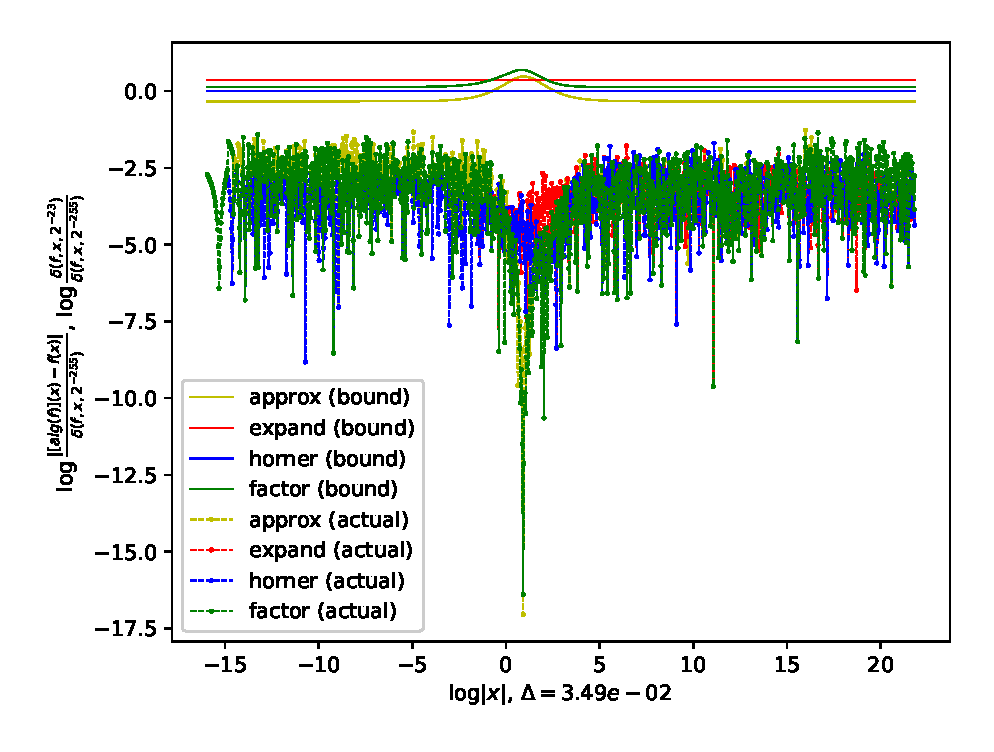
\includegraphics[width=\linewidth]{figs/1}
  		\caption{$4x^4-44x^3+61x^2+270x-525$}
  		\label{fig:sub1}
	\end{subfigure}%
	\begin{subfigure}{.5\textwidth}
  		\centering
		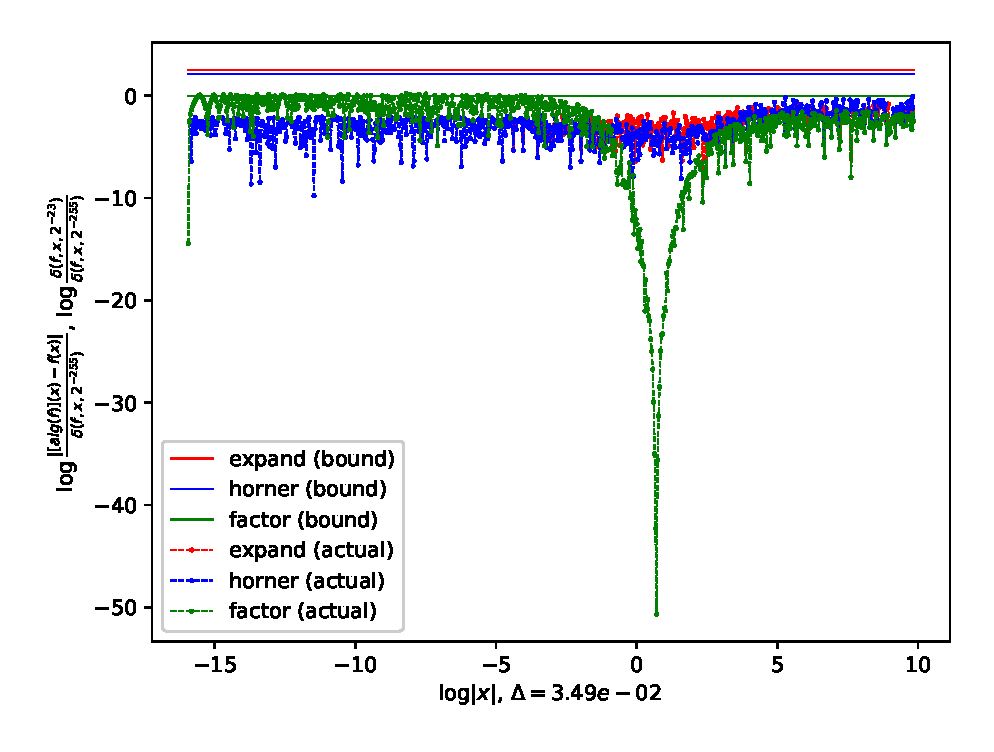
\includegraphics[width=0.95\linewidth]{figs/2}
		\caption{$(x-2)^9$}
  		\label{fig:sub1}
	\end{subfigure}%
	\iffalse
	\begin{subfigure}{.5\textwidth}
  		\centering
		\includegraphics[width=\linewidth]{figs/5}
  		\caption{$(x - 1)(x - 923)(x - 2039822)(x - 23029832)$}
  		\label{fig:sub2}
	\end{subfigure}
	\fi
\end{figure*}
An analysis of the actual error bounds shown in Figure 3 indicates that the predicted theoretical bounds do contain the true error values.
While this bound is equivalent to an optimistic bound for Horner's form, the bound can still be improved for factored form near roots.
Observe that in Figure 3 the true error is less near the roots, while the predicted bound for factored form has a bump at the same location.
Also observe that some polynomials are piecewise optimal with Horner form best in one interval and factor form better on a different region of the interval.
In a follow up paper, a more detailed local analysis of the error bound for factored form will be provided in comparison with the bound proved in this paper, where the bounds near roots of factored form terms will be investigated.

\begin{example}
	Consider the expression $f$ from figure 3(a).
	%such that $\mc E(f) = 4x^4-44x^3+61x^2+270x-525$. Then the corresponding sets are $S(\mc E(f)) = \set{4,-44,61,270,-525}$ and $P(\mc E(f)) = \set{4,3,2}$. 
	The appropriate form is $\mc H(f)$.
	$$\begin{array}{c|cccc}
		& \mc E(f) & \mc H(f) & \mc F(f) & \mc R(f) \\
	%	\hline
	%\nu(f) & 126.85906848480876 & 27.659637207554205 & 28.555467999782095 \\
	%E(f,\epsilon,\Delta) & 41022.83760836261 & 40954.94019676484 & 40981.689093380344
	(c,\sigma,\conj s,\conj p) & (10, 2.228, 4.228, 3.0) & (7, 1.687, 3.951, 1.0) & (8, 0.861, 1.785, 2.0) & (5, 0.595, 1.337, 2.0) \\
	\nu(f) & 92.0863245436194 & 18.073187517116104 & 19.83687735202171 & 8.923106875013321 \\
	\Phi(f,\epsilon,\Delta) & 1.029960829726364 & 0.9999999667868625 & 1.0148546060152759 & 0.9778483323687441 \\
	\text{bytes} & 3014.7186666666666 & 185.24666666666667 & 156.549 & 173.35433333333333
	\end{array}. $$
\end{example}

\iffalse
\begin{figure*}[h]
	\centering
\caption{Two unequal polynomial terms using identical coefficients and exponents}% can have opposite error characteristics near their roots}
	\begin{subfigure}{.5\textwidth}
  		\centering
		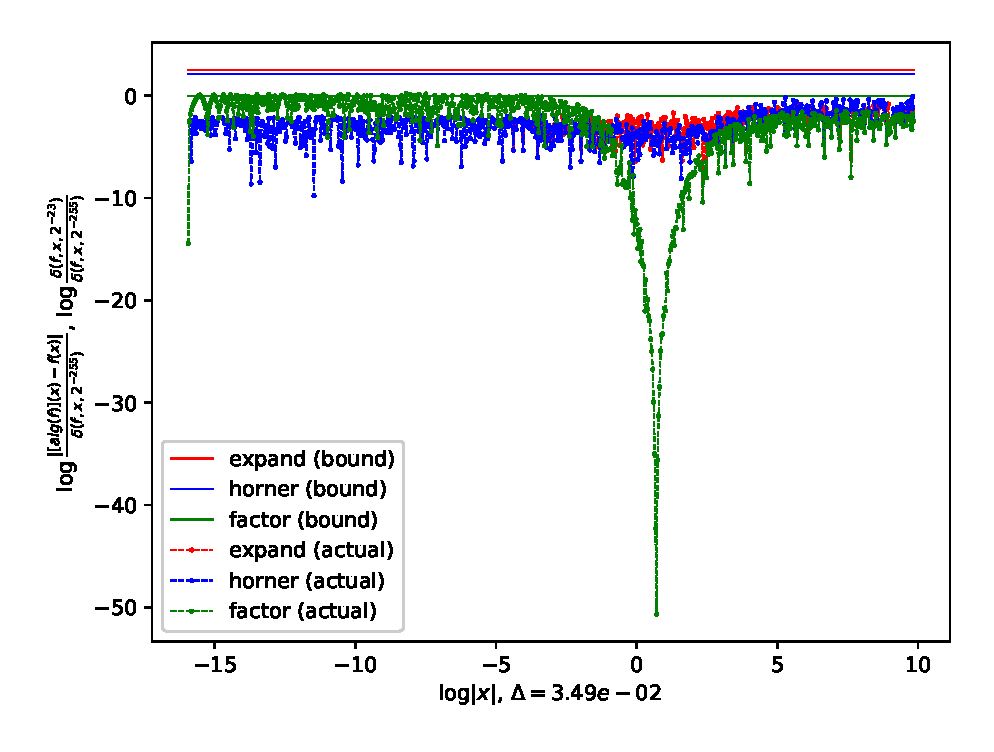
\includegraphics[width=0.95\linewidth]{figs/2}
		\caption{$(x-2)^9$}
  		\label{fig:sub1}
	\end{subfigure}%
	\begin{subfigure}{.5\textwidth}
  		\centering
		\includegraphics[width=0.95\linewidth]{figs/3}
  		\caption{$x^9-2$}
  		\label{fig:sub2}
	\end{subfigure}
\end{figure*}
\fi

\begin{example}
	Consider the expression $f$ from figure 3(b).
	The appropriate form is $\mc F(f)$.
	$$\begin{array}{c|cccc}
		& \mc E(f) & \mc H(f) & \mc F(f) \\
	%	\hline
		(c,\sigma,\conj s,\conj p) & (25, 3.212, 6.810, 5.5) & (17, 1.340, 6.810, 1.0) & (2, 1.504, 0.693, 9.0) \\
		\nu(f) & 643.1128014851948 & 51.3441179785937 & 18.378934415299785 \\
		\Phi(f,\epsilon,\Delta) & 1.2735710938627083 & 1.2317985884634024 & 1.0000000140002385 \\
		\text{bytes} & 3135.4363333333336 & 240.71133333333333 & 98.13
	\end{array}. $$
\end{example}

The source code that generated the results in this paper can be obtained from \textit{Wilkinson.jl} \cite{chakravala-wilkinson} package along with the source for the paper, which will be distributed using the \textit{VerTeX.jl} format.
\begin{verbatim}
using Reduce, Wilkinson; import SyntaxTree: exprval
PolynomialComparison(polyexpand(:x,[-525,270,61,-44,4]))
PolynomialComparison(polyfactors(:x,2ones(9)))
PolynomialComparison(:(x^9-2))
PolynomialComparison(polyfactors(:x,[23029832,2039822,923,1]))
PolynomialComparison(Algebra.prod(:((x+n)^n),:n,1,5))
PolynomialComparison(:((((x - 1) ^ 2 * x ^ 2 - 1) ^ 2 - 1) ^ 2))
\end{verbatim}

Evaluating \verb`PolynomialComparison` objects computes the listed data, which can be displayed with \verb`plot` using the \textit{PyPlot.jl} package by default.
Note that all the global characteristic values are the optimal when minimized (for $\nu,\Phi$, memory allocation, etc.).
Typically, the expanded form requires significantly more memory consumption, while the factored and Horner form are the most competitive. Sometimes, the rounded roots form does very well also, but the numerical error depends on the accuracy of the roots used.

\begin{example}
	Consider the expression $x^9-2$.
	The appropriate form is $\mc H(f)$.
	$$\begin{array}{c|cccc}
		& \mc E(f) & \mc H(f) & \mc R(f) \\
	%	\hline
		(c,\sigma,\conj s,\conj p) & (2, 1.504, 0.693, 9.0) & (2, 1.504, 0.693, 9.0) & (24, 0.481, -0.446, 1.0) \\
		\nu(f) & 18.378934415299785 & 18.378934415299785 & 11.11841280417285 \\
		\Phi(f,\epsilon,\Delta) & 1.000000041184039 & 1.000000041184039 & 1.5646134826064557 \\
		\text{bytes} & 2931.4513333333334 & 97.98633333333333 & 1948.7503333333334
	\end{array}. $$
\end{example}

\iffalse
\begin{figure*}[h]
	\centering
	\caption{Sometimes different sections of the interval have a piecewise varying optimal form}
	\begin{subfigure}{.5\textwidth}
  		\centering
		\includegraphics[width=\linewidth]{figs/4}
  		\label{fig:sub1}
	\end{subfigure}%
	\begin{subfigure}{.5\textwidth}
  		\centering
		\includegraphics[width=\linewidth]{figs/6}
  		\caption{$(((x - 2) ^ 2 x ^ 2 - 1) ^ 2 - 1) ^ 2$}
  		\label{fig:sub2}
	\end{subfigure}
\end{figure*}
\fi

\begin{example}
	Consider the expression $(x - 1)(x - 923)(x - 2039822)(x - 23029832)$, appropriate form is $\mc F(f)$.
	$$\begin{array}{c|cccc}
		& \mc E(f) & \mc H(f) & \mc F(f) \\
	%	\hline
		(c,\sigma,\conj s,\conj p) & (10, 18.39, 31.28, 3.0) & (7, 7.091, 31.28, 1.0) & (5, 6.679, 9.827, 1.0) \\
		\nu(f) & 719.5002771106713 & 104.26001750963377 & 40.50789575171883 \\
		\Phi(f,\epsilon,\Delta) & 1.0218699473050092 & 1.0106162581578118 & 0.9999999990283254 \\
		\text{bytes} & 3002.5823333333333 & 147.319 & 142.482
	\end{array}. $$
\end{example}
% (((x - 2) ^ 2 * x ^ 2 - 1) ^ 2 - 1) ^ 2

\begin{example}
	Consider the expression $\ds\prod_{n=1}^7 (x+n)^n$.
	The appropriate form is $\mc F(f)$.
	$$\begin{array}{c|cccc}
		& \mc E(f) & \mc H(f) & \mc F(f) \\
	%	\hline
		(c,\sigma,\conj s,\conj p) & (55, 19.81, 28.78, 15.0) & (55, 6.867, 28.78, 1.0) & (14, 0.558, 1.3607, 4.5) \\
		\nu(f) & 19699.29024455475 & 773.2300130297801 & 54.944165783862005 \\
		\Phi(f,\epsilon,\Delta) & 1.0096353233930733 & 1.0096353233930733 & 1.0 \\
		\text{bytes} & 6451.475333333334 & 600.759 & 378.9683333333333
	\end{array}. $$
\end{example}
\begin{example}
	Consider the expression $(((x-2)^2x^2-1)^2-1^2)$.
	The appropriate form is $\mc F(f)$.
	$$\begin{array}{c|ccccc}
		& \mc E(f) & \mc H(f) & \mc F(f) & \mc R(f) & \mc O(f) \\
	%	\hline
		(c,\sigma,\conj s,\conj p) & (35, 1.0, 3.1, 6.75) & (25, 0.7, 3.1, 4.0) & (12, 0.4, 0.7, 3.1) & (15, 0.5, 0.09, 2.0) & (8, 0.7, 1.0, 2.0) \\
		\nu(f) & 427.8418916234 & 152.3413216001 & 21.59664312746 & 6.93957471367 & 13.3341854087 \\
		\Phi(f,\epsilon,\Delta) & -4.3314048550 & -4.41216949054 & -4.58108950145 & 1.035101808575 & 0.999999969189 \\
		\text{bytes} & 3455.111 & 287.113666667 & 178.6336666667 & 1484.140333333 & 129.7606666668
	\end{array}. $$
\end{example}

\begin{remark}
	Occasionally the $\Phi$ value is negative, which might seem surprising but this value is fully consistent with the theoretical and local true error bound data, the behavior of which will be discussed and explored in greater detail in the follow up paper.
\end{remark}

The numerical data provided in the examples should help clarify why the expression value formula is defined the way it is. Observe that for expanded form, the operation count is typically very high along with the average exponent, while these values are smaller in Horner form. 
If the term can be factorized with real roots (exact or approximated) then expression value may be improved further.
The \verb+factor+ algorithm provided by \textit{Reduce.jl} does not automatically round the roots and hence can only provide a semi-factored form in some scenarios, as in Example 2. In these cases, the Horner form is more appropriate.

\newpage
\section{Conclusion}
When a randomized polynomial is constructed, it is procedurally generated using its form's recursive abstract syntax tree constructor. For forms like factorized and Horner, and some others, it is typically found that the particular randomized term is most optimal in the same form it was \say{generated in,} since the form is simplest.
%Another such an example is the recursive method $b_j \mapsto \widehat{\ \ }(-(1,b_j(x,g_*,\dots),2)$, for which the original forms turn out to be significantly more optimal.
%However, to an inverse algorithm that is rewriting a scrambled expression back into such an arbitrary form, it might be an inaccessible form.
By studying the characteristics of each method, a more efficient construct of code generation can be applied to numerical basis polynomials.
Results indicate $\nu(\mc H(f)) \leq \nu(\mc F(f))$ if and only if $\Xi(f,\epsilon,\Delta)\geq0$ with a 100.0\% agreement rate,
 implying that the simpler method is able to succesfully select for the optimal polynomial form to minimize error propagation measured in the more cumbersome integration.
Based on the results from the analysis, the recommended algorithm for selecting the optimal form is:
\begin{verbatim}
optimal(expr) = (h=horner(expr); f=factor(h); exprval(h)[1] <= exprval(f)[1] ? h : f)
\end{verbatim}
Due to the computational simplicity of the expression value method in comparison to the floating point error bound Simpson-Stieltjes integral estimation method, the expression value method is the demonstrably faster, more efficient, and equally reliable method for determining the optimal expression form characterization.
Some of the possible applications where an optimal polynomial form might be useful include the differential geometric algebra of the \textit{Grassmann.jl} package, in which the multivariate \textit{Leibniz.jl} Taylor polynomial forms are manipulated via operator algebras of tensor fields acting on differential forms \cite{grassmann-juliacon-2019}.

%(+Acknowledgements)

\textbf{Acknowledgements}:
Thanks to Thomas Lewis for discussing the results, Filip Saidak for suggestions,  and Maya Chhetri for teaching the Stieltjes integral.
Thanks to Nathan Smith from the Julia community and Arthur Norman and Eberhart Shruefer from the Reduce developer team for answering questions and collaborating on the software that enabled the creation of the \textit{Reduce.jl} software.
%Many thanks to my family for supporting this research.

\iffalse
\begin{example}
	The following compares the calculations for various forms of a polynomial:
	%\begin{align*}
	%	e &= 4x^4-44x^3+61x^2+270x-525 \\
	%	e_f &= ((x^2-6x)-21)\cdot(2x-5)^2 \\
	%	e_H &= ((4(x-11)x+61)x+270)x-525
	%\end{align*}
	\begin{align*}
		c(e) &= 11, & c(e_f) &= 9, & c(e_H) &= 8, \\
		n(e) &= 6, & n(e_f) &= 5, & n(e_H) &= 6, \\
		m(e) &= 3, & m(e_f) &= 2, & m(e_H) &= 0, \\
		\sum_{s\in S(e)}\log s &= 4.291391377798259, & \sum_{s\in S(e)}\log s &= 2.348807437186723, & \sum_{s\in S(e)}\log s &= 4.060342317611611, \\
		\sum_{p\in P(e)}p &= 3.0, & \sum_{p\in P(e)}p &= 2.0, & \sum_{p\in P(e)}p &= 1.0, \\
		v(e) &= 141.61591546734255, & v(e_f) &= 42.27853386936101, & v(e_H) &= 32.48273854089289
	\end{align*}
\end{example}
%\iffalse
\begin{example}
	\begin{align*}
		e_f &= \left(x+7\right)^{7} \left(x+6\right)^{6} \left(x+5\right)^{5} \left(x+4
		\right)^{4} \left(x+3\right)^{3} \left(x+2\right)^{2} \left(x+1\right)
	\end{align*}
	\iffalse
	\begin{align*}
		e_H &= (((((((((((((
		((((((((((((( \\
		&(x+140) x+9408) x+404012) x+12452860) x+293354100 \\
		&) x+5491243184) x+83839010860) x+1063406184918) x+ \\
		&11355388042796) x+103080193140016) x+801097015860804) x+ \\
		&5356632994052156) x+30917671615556572) x+154307800127905488) \\
		&x+666179931589106948) x+2485349318616140689) x+ \\
		 &7993549830308360568) x+22077583830099907600) x+ \\
		&52067305426360848992) x+104039758639368727776) x+ \\
		&174299255833816957824) x+241386405085113410304) x+ \\
		&271057611231886800384) x+240180965385332025600) x+ \\
		&161326036746072576000) x+77030436760058880000) x+ \\
		&23238364791398400000) x+3319766398771200000
	\end{align*}
	\fi
	\begin{align*}
		c(e_f) &= 14, & c(e_H) &= 55, \\
		n(e_f) &= 7, & n(e_H) &= 18, \\
		m(e_f) &= 6, & m(e_H) &= 0, \\
		\sum_{s\in S(e)}\log s &= 1.2178801944379163, & \sum_{s\in S(e)}\log s &= 28.78242520303318, \\
		\sum_{p\in P(e)}p &= 4.5, & \sum_{p\in P(e)}p &= 1.0, \\
		v(e_f) &= 76.72645224958872, & v(e_H) &= 1583.033386166825
	\end{align*}
\end{example}
\fi

\bibliography{poly}
\bibliographystyle{plain}

\end{document}
